\documentclass[12pt]{article}

\input preamble

\title{Principles of Parallel Architecture\\
Project Report 2}
\author{Xitong Liu \\
xliu@ece.udel.edu}

\begin{document}

\maketitle

\section{Introduction}
In this report, we will introduce the methods applied to optimize
the performance of Matrix Multiplication on parallel architecture.
Results showed that the performance has been improved a lot comparing
to the baseline approach proposed in the previous report.

\section{Baseline}
The setup of the baseline parallel is straightforward, as we divide
one matrix operand evenly into several parts, each part is distributed
to one thread. The approach is shown in Figure~\ref{fig:matrix-divide}.

\begin{figure}[h!]
	\begin{center}
		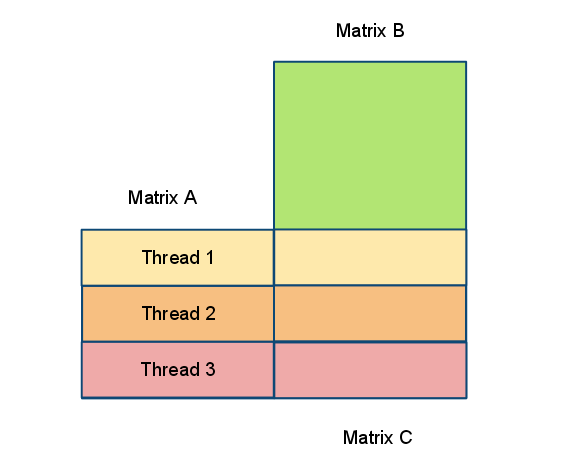
\includegraphics[width=0.5\textwidth]{matrix-divide.png}
		\caption{\label{fig:matrix-divide}Matrix Division}
	\end{center}
\end{figure}

\section{Cache Line}
In the baseline version, for $\mathbf{C}=\mathbf{A}\times\mathbf{B}$,
in the inner most loop, $\mathbf{A}$ is accessed in a row major. When 
the first element of one row in $\mathbf{A}$ is accessed, the access 
to the following elements can benefit from the cache line since they
are adjacent in memory and loaded in the same cacheline. However, 
$\mathbf{B}$ is accessed in a column major and the access of the 
following elements may cause more loads of cache line. The sample code 
for $\mathbf{C}=\mathbf{A}\times\mathbf{B}$ is shown as below:

\begin{verbatim}
DO I = 1, N 
  DO J = 1, N
	  C(I,J) = 0.0 
      DO K = 1, N
      C(I,J) = C(I,J) + A(I,K) * B(K,J) 
    ENDDO
  ENDDO
ENDDO
\end{verbatim}

We transpose $\mathbf{B}$ to $\mathbf{B^{T}}$ at first. In the 
following multiplication operation's inner most loop, access of 
both $\mathbf{A}$ and $\mathbf{B^{T}}$ is in row major and both
of them can benefit from the acceleration of cache line. More 
detail is depicted in Figure~\ref{fig:cacheline}. The sample code 
is shown as below:

\begin{verbatim}
DO I = 1, N 
  DO J = 1, N
	  C(I,J) = 0.0 
      DO K = 1, N
      C(I,J) = C(I,J) + A(I,K) * BT(J,K) 
    ENDDO
  ENDDO
ENDDO
\end{verbatim}

\begin{figure}[h!]
	\begin{center}
		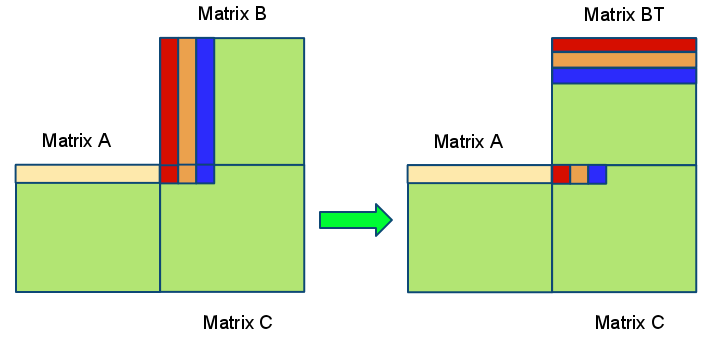
\includegraphics[width=0.7\textwidth]{cacheline.png}
		\caption{\label{fig:cacheline}Matrix Transpose}
	\end{center}
\end{figure}

\section{SSE}
Streaming SIMD Extension (SSE) is a SIMD instruction set 
introduced by Intel, begin in Pentium III product line. 
\footnote{http://en.wikipedia.org/wiki/Streaming\_SIMD\_Extensions}
It adds eight new 128-bit registers to the CPU, known as XMM0 
through XMM7. On Intel 64 platform, in which the experiment is 
conducted, the registered have been extended from XMM0 to XMM15.
Each register can hold 128 bit data, e.g. four 32-bit single-precision
floating point numbers, or two 64-bit double-precision floating point
numbers. Specific floating operation instructions can be issued in a
separate FPU and they can operation on the whole 128-bit register.
With the help of SSE, the floating operation instructions can be
executed in parallel with other instructions which may lead great 
performance boost in pipelining. 

GCC has built-in support for SSE, and all the SSE instructions
are encapsulated in built-in functions started with 
\texttt{\_\_builtin\_ia32}. The code snippet is shown as below:

\footnotesize
\begin{verbatim}
// SSE
typedef float v4sf __attribute__ ((vector_size(16)));
#define SSE_LENGTH 4

v4sf acc;
v4sf oprand_a;
v4sf oprand_b;
ftype imd_ret[SSE_LENGTH];

for(cycleI = start; cycleI < end; ++ cycleI){
  for(cycleJ = 0; cycleJ < matrixB.xDim; ++ cycleJ){
  // set acc to 0
  acc = __builtin_ia32_loadups(init_array);
        
  for(cycleK = 0; cycleK < (dim - SSE_LENGTH + 1); cycleK += SSE_LENGTH){
    oprand_a = __builtin_ia32_loadups(&(matrixA.data[cycleI * dim + cycleK]));
    oprand_b = __builtin_ia32_loadups(&(matrixBT.data[cycleJ * dim + cycleK]));
    acc = __builtin_ia32_addps(acc, __builtin_ia32_mulps(oprand_a, oprand_b));
  }
  __builtin_ia32_storeups(imd_ret, acc);

  for(cycleK = 1; cycleK < SSE_LENGTH; ++ cycleK){
    imd_ret[0] += imd_ret[cycleK];
  }
  matrixC.data[cycleI * dim + cycleJ] = imd_ret[0];
}
\end{verbatim}
\normalsize

\texttt{v4sf} is defined as vector type which is composed of 4 single-precision
floating point numbers and it is stored in XMM registers. 
\texttt{\_\_builtin\_ia32\_loadups} is used to load data from main memory to 
XMM registers, and \texttt{\_\_builtin\_ia32\_storeups} are used to store the 
data from XMM registers to main memory. \texttt{\_\_builtin\_ia32\_addps} and 
\texttt{\_\_builtin\_ia32\_mulps} is used for XMM add and multiply operation 
respectively. Since each operation can manipulate 4 float numbers a time, the 
stride of the inner most loop is set to 4.

\section{Unrolling and Scheduling}
To better utilize the benefits of the pipelining, we apply unrolling and scheduling.
Considering the limitation that there are 16 XMM registers per core, we unroll the
inner loop by 4 steps and reschedule the execution order to hide the load and
store latency. The code snippet is shown as below:

\footnotesize
\begin{verbatim}
for(cycleK = 0; cycleK < (dim - SSE_LENGTH + 1); cycleK += SSE_LENGTH){
  oprand_a = __builtin_ia32_loadups(&(matrixA.data[cycleI * dim + cycleK]));

  oprand_b_0 = __builtin_ia32_loadups(&(matrixBT.data[cycleJ * dim + cycleK]));
  oprand_b_1 = __builtin_ia32_loadups(&(matrixBT.data[(cycleJ + 1) * dim + cycleK]));
  oprand_b_2 = __builtin_ia32_loadups(&(matrixBT.data[(cycleJ + 2) * dim + cycleK]));
  oprand_b_3 = __builtin_ia32_loadups( &(matrixBT.data[(cycleJ + 3) * dim + cycleK]));
          
  acc_0 = __builtin_ia32_addps(acc_0, __builtin_ia32_mulps(oprand_a, oprand_b_0));
  acc_1 = __builtin_ia32_addps(acc_1, __builtin_ia32_mulps(oprand_a, oprand_b_1));
  acc_2 = __builtin_ia32_addps(acc_2, __builtin_ia32_mulps(oprand_a, oprand_b_2));
  acc_3 = __builtin_ia32_addps(acc_3, __builtin_ia32_mulps(oprand_a, oprand_b_3));
}
\end{verbatim}
\normalsize

\section{Software Pipelining}
We also tried software pipelining to pursue further performance improvement. 
The approach is intuitive, as shown as below:
\footnotesize
\begin{verbatim}
int is_odd = 0;

for(cycleI = start; cycleI < end; ++ cycleI){
  for(cycleJ = 0; cycleJ < matrixB.xDim - 1; cycleJ += 2){

    for(cycleK = SSE_LENGTH; cycleK < (dim - SSE_LENGTH + 1); 
      cycleK += SSE_LENGTH){
      
      is_odd = cycleK / 4;
      is_odd = is_odd % 2;
        
      if(is_odd){
        prefetch data of group 1 for the next run;
        do accumulation on group 0;
      }else{
        prefetch data of group 0 for the next run;
        do accumulation on group 1;
      }
    }
        
    // calculate the sum for the last run
    if(!is_odd){
    	  do accumulation on group 0;
    }else{
      do accumulation on group 1;
    }
    store the result to matrixC;
  }
}
\end{verbatim}
\normalsize

We prepared 2 group of registers. In the loop iteration, we load data 
into one group of registers and do calculation on the other group so that
the data loading latency can be hiden by pipelining.

\section{Experiment Results}
We apply different optimization methods step by step and the experiment setup 


\end{document}

\begin{comment}
\begin{figure}[h!]
	\begin{center}
		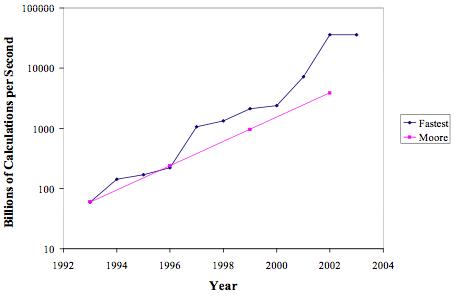
\includegraphics[width=0.7\textwidth, angle=0]{fatest.png}
		\caption{\label{fig:fatest}Fatest SuperComputer in the world}
	\end{center}
\end{figure}
\end{comment}